\documentclass[tikz,border=2pt]{standalone}
\usepackage{amsmath}
\usepackage{pgfplots}
\pgfplotsset{compat=1.18}
\usetikzlibrary{arrows.meta}
\begin{document}
% Sector K={0<=x2<=x1} contains (1,0),(1,1) and every nonnegative combination of them,
% e.g. 2(1,0)+3(1,1)=(5,3), built as the parallelogram on 2(1,0)=(2,0) and 3(1,1)=(3,3).
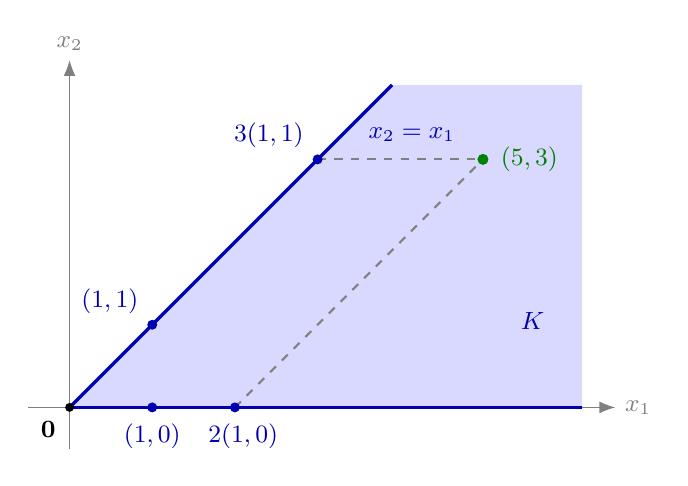
\begin{tikzpicture}[font=\small, >={Latex[length=2mm]}, x=1.05cm, y=1.05cm]
  \fill[blue!15] (0,0) -- (6.2,0) -- (6.2,3.9) -- (3.9,3.9) -- cycle;
  \draw[gray, ->] (-0.5,0) -- (6.6,0) node[anchor=west] {$x_1$};
  \draw[gray, ->] (0,-0.5) -- (0,4.2) node[anchor=south] {$x_2$};
  \draw[blue!70!black, very thick] (0,0) -- (6.2,0);
  \draw[blue!70!black, very thick] (0,0) -- (3.9,3.9);
  \node[blue!70!black, anchor=north west] at (3.5,3.5) {$x_2=x_1$};
  \node[blue!70!black] at (5.6,1.05) {$K$};
  \draw[gray, thick, dashed] (2,0) -- (5,3);
  \draw[gray, thick, dashed] (3,3) -- (5,3);
  \fill (0,0) circle (1.6pt);
  \node[anchor=north east] at (-0.05,-0.05) {$\boldsymbol{0}$};
  \fill[blue!70!black] (1,0) circle (1.8pt);
  \node[blue!70!black, anchor=north] at (1,-0.08) {$(1,0)$};
  \fill[blue!70!black] (2,0) circle (1.8pt);
  \node[blue!70!black, anchor=north] at (2.1,-0.08) {$2(1,0)$};
  \fill[blue!70!black] (1,1) circle (1.8pt);
  \node[blue!70!black, anchor=south east] at (0.95,1.02) {$(1,1)$};
  \fill[blue!70!black] (3,3) circle (1.8pt);
  \node[blue!70!black, anchor=south east] at (2.95,3.02) {$3(1,1)$};
  \fill[green!50!black] (5,3) circle (2pt);
  \node[green!50!black, anchor=west] at (5.1,3) {$(5,3)$};
\end{tikzpicture}
\end{document}
